\section{Three further findings}
\label{sec:three-further-findings}

% Generated by `uv run python -m gainpred.writeup`; do not edit by hand.
\begin{table}[htbp]
\centering
\caption{Agreement rule minus no-carry rule after round 4, points, evaluation
  runs: mean over three starting models and worst single run (its starting
  model).}
\label{tab:passmark}
\small
\begin{tabular}{lrrrr}
\toprule
Digits & Mean gap & Worst run & Mean gap, carry & Worst run, carry \\
\midrule
8 & -0.2 & -0.5 (4) & -0.4 & -0.9 (4) \\
9 & -0.3 & -0.7 (4) & -0.4 & -1.1 (4) \\
10 & -0.3 & -0.8 (4) & -0.5 & -1.4 (4) \\
11 & -0.4 & -1.1 (4) & -0.5 & -1.3 (4) \\
12 & -0.5 & -1.3 (4) & -0.8 & -2.2 (4) \\
13 & -0.5 & -1.0 (4) & -1.0 & -1.8 (4) \\
14 & -0.8 & -1.8 (4) & -1.3 & -3.1 (4) \\
15 & -0.5 & -1.2 (4) & -1.1 & -2.2 (4) \\
\bottomrule
\end{tabular}
\end{table}

% Generated by `uv run python -m gainpred.writeup`; do not edit by hand.
\begin{table}[t]
\centering
\caption{Share (\%) of kept training answers that carry out of a place, by kind of place, in the round the length is first trained on; mean over starting points 2-4. NC: no-carry rule; AG: agreement rule.}
\label{tab:carries}
\small
\begin{tabular}{lrrrrrr}
\toprule
Digits & NC: cut 1 & NC: other cuts & NC: no cut & AG: cut 1 & AG: other cuts & AG: no cut \\
\midrule
8 & 0.0 & 55.1 & 48.6 & 22.1 & 27.8 & 46.9 \\
9 & 0.0 & 57.8 & 47.7 & 28.0 & 24.6 & 47.5 \\
10 & 0.0 & 54.9 & 49.2 & 22.3 & 27.4 & 48.3 \\
11 & 0.0 & 57.8 & 48.5 & 28.5 & 24.6 & 48.4 \\
12 & 0.0 & 54.9 & 49.3 & 22.3 & 27.5 & 48.6 \\
13 & 0.0 & 59.4 & 48.9 & 29.7 & 45.8 & 48.3 \\
14 & 0.0 & 59.8 & 48.9 & 25.8 & 43.1 & 48.1 \\
15 & 0.0 & 58.1 & 48.7 & 37.8 & 38.7 & 47.6 \\
\bottomrule
\end{tabular}
\end{table}

% Generated by `uv run python -m gainpred.writeup`; do not edit by hand.
\begin{table}[htbp]
\centering
\caption{What the filter removes and whether the student learns it anyway,
  evaluation runs, in the round that first trains each length. Kept: share (\%)
  of kept training answers with a carry out of the split-1 place. Carry:
  accuracy (\%) on the study group with a carry across split 1, before and after
  the round (mean over the evaluation runs; lowest in brackets). No-carry: the
  other group after. NC: no-carry rule; AG: agreement rule. Defined after the
  evaluation runs.}
\label{tab:filter_gap}
\small
\resizebox{\linewidth}{!}{%
\begin{tabular}{lrrrrrrrr}
\toprule
Digits & NC kept & NC carry before & NC carry after & NC no-carry after
  & AG kept & AG carry before & AG carry after & AG no-carry after \\
\midrule
8 & 0.0 & 13.6 & 99.5 (99.0) & 99.8 & 22.1 & 13.6 & 99.3 (98.1) & 99.9 \\
9 & 0.0 & 0.0 & 99.0 (97.2) & 99.8 & 28.0 & 0.0 & 98.6 (96.3) & 99.7 \\
10 & 0.0 & 58.6 & 99.2 (97.7) & 99.7 & 22.3 & 83.1 & 98.9 (97.4) & 99.9 \\
11 & 0.0 & 0.1 & 99.2 (97.7) & 99.6 & 28.5 & 0.0 & 98.9 (97.0) & 99.3 \\
12 & 0.0 & 79.1 & 99.4 (98.4) & 99.9 & 22.3 & 97.4 & 98.9 (96.6) & 99.6 \\
13 & 0.0 & 0.7 & 99.0 (97.4) & 99.7 & 29.7 & 6.7 & 98.5 (96.2) & 99.6 \\
14 & 0.0 & 92.0 & 99.4 (98.3) & 99.7 & 25.8 & 97.3 & 98.1 (95.2) & 99.5 \\
15 & 0.0 & 0.4 & 99.4 (98.4) & 99.7 & 37.8 & 4.6 & 98.4 (96.2) & 99.7 \\
\bottomrule
\end{tabular}
}
\end{table}

% Generated by `uv run python -m gainpred.writeup`; do not edit by hand.
\begin{figure}[htbp]
\centering
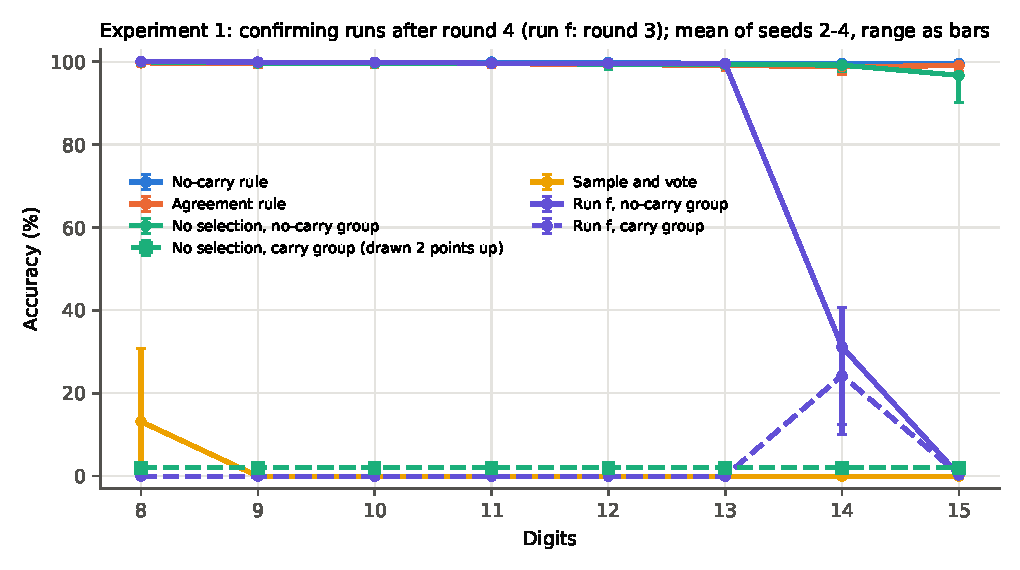
\includegraphics[width=\linewidth]{generated/figure_exp1.pdf}
\caption{Accuracy after round 4 (no selection after the no-carry rule: after its
  one round, round 3), evaluation runs; mean over the three starting models,
  range as bars.}
\label{fig:exp1}
\end{figure}

% Generated by `uv run python -m gainpred.writeup`; do not edit by hand.
\begin{table}[htbp]
\centering
\caption{Longest run, one round: accuracy (\%) on the test problems, all groups
  and crossing runs of 5-8; mean over the evaluation runs (lowest-highest). All
  pools ten groups of 1,000 problems, nine of which contain a crossing run.}
\label{tab:exp2}
\small
\resizebox{\linewidth}{!}{%
\begin{tabular}{lrrrrr}
\toprule
Teacher & All & Crossing run 5 & Crossing run 6 & Crossing run 7
  & Crossing run 8 \\
\midrule
Before & 53.5 (46.3--58.0) & 57.3 (19.1--78.2) & 1.5 (0.0--4.5) & 0.0 (0.0--0.0)
  & 0.0 (0.0--0.0) \\
Join at the split & 98.0 (96.9--98.6) & 99.2 (98.3--99.7) & 99.4 (99.0--99.7)
  & 97.1 (96.3--98.1) & 91.5 (85.6--94.9) \\
Edges-differ rule & 53.4 (53.0--53.9) & 44.0 (39.6--47.7) & 0.0 (0.0--0.0)
  & 0.0 (0.0--0.0) & 0.0 (0.0--0.0) \\
Pick the longer & 23.6 (22.6--24.4) & 0.0 (0.0--0.0) & 0.0 (0.0--0.0)
  & 0.0 (0.0--0.0) & 0.0 (0.0--0.0) \\
Join at the split, withheld & 75.1 (74.9--75.6) & 98.3 (97.7--98.8)
  & 98.0 (96.8--99.5) & 0.0 (0.0--0.0) & 0.0 (0.0--0.0) \\
\bottomrule
\end{tabular}
}
\end{table}

% Generated by `uv run python -m gainpred.writeup`; do not edit by hand.
\begin{figure}[htbp]
\centering
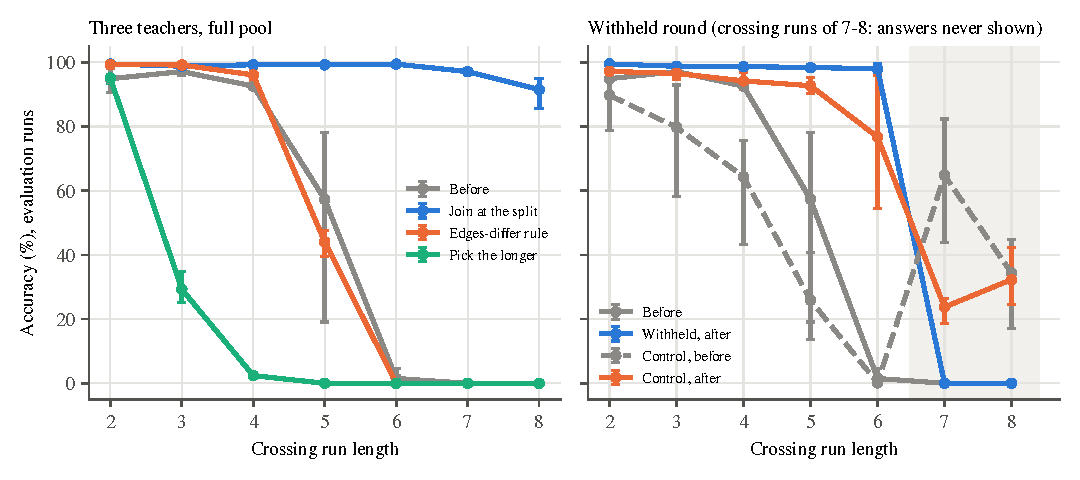
\includegraphics[width=\linewidth]{generated/figure_exp2.pdf}
\caption{Longest run: accuracy by joined run length before and after one round,
  evaluation runs.}
\label{fig:exp2}
\end{figure}

% Generated by `uv run python -m gainpred.writeup`; do not edit by hand.
\begin{table}[htbp]
\centering
\caption{The withheld version (join at the split, trained without crossing runs
  whose left part is 3-4), evaluation runs: accuracy (\%) before $\rightarrow$
  after the round, lowest-highest over the three starting models. Left part: how
  many symbols of the crossing run lie in the left piece. The teacher shows
  crossing runs of 6 with left part 1-2, never with left part 3-4, and never an
  answer of 7 or 8 on long strings.}
\label{tab:withheld}
\small
\begin{tabular}{lrr}
\toprule
Test problems & Problems & Before $\rightarrow$ after \\
\midrule
Shown combinations: crossing run of 6, left part 1-2 & 478
  & 0.0--5.9 $\rightarrow$ 96.7--98.3 \\
Withheld combinations: crossing run of 6, left part 3-4 & 877
  & 0.0--4.0 $\rightarrow$ 96.6--99.7 \\
Answers never shown: crossing runs of 7-8 & 2,000
  & 0.0--0.0 $\rightarrow$ 0.0--0.0 \\
\bottomrule
\end{tabular}
\end{table}


% Section 5, filter-gap paragraph:
% The same effect has been reported outside self-improvement: when the
% training signal for a skill is withheld, language models still learn much
% of it from the rest of their data \citep{marosi2026general}. Our withheld
% test marks where this stops: the student learns what appears elsewhere in
% the teacher's output, and nothing that never appears.

% Section 6, table of published loops, two rows:
% BaseRSI \citep{zhang2026basersi}: differ = the teacher-student gap is the
%   training signal; correct = acceptance test on labelled questions;
%   lacks = by construction (the teacher has the harness entry).
%   Needs: labelled validation questions.
% AeroRSI \citep{wu2026aerorsi}: differ = a repair is kept only where the
%   original action fails; correct = the policy must complete the flight from
%   the repair in a simulator (unverified repairs help little or hurt);
%   lacks = rule-based proposals are added because the policy often cannot
%   sample the action it needs. Needs: a simulator.

% Section 7, discussion:
% Piccolo \citep{piccolo2026} reports that falling loss can come with worse
%   accuracy: a caution against cheap signals taken during training.
% A calibrated judge can replace reference answers as a training signal
%   \citep{agnihotri2026calibrated}, but needs a much larger second model and
%   about a hundred labels, and is overconfident on problems the base model
%   mostly fails.
